\section{Du génome aux processus cellulaires : exploration fonctionnelle}

\subsection{Gènes : Régulations et fonctions}
\label{sec:fn_reg}

Les réactions qui se produisent dans les cellules procaryotes sont souvent complexes et impliquent une multitude de réactifs et de produits. Toutes ces réactions nécessitent la présence de protéines spécifiques pour être réalisées. Ces protéines sont produites et dégradées par la cellule en fonction des conditions rencontrées. C'est pourquoi l'information est stockée dans une structure durable et transmissible, le gène. Chaque gène sera transcrit en une molécule d'ARN messager (ARNm) par l'ARN polymérase, qui sera traduite en protéine par le ribosome (impliquant l'ARNr et l'ARNt). 


Dans une cellule, les protéines ont un temps de "vie" allant de quelques minutes à quelques heures. Il est donc nécessaire de produire les protéines régulièrement, toutefois cette production à un coût pour la cellule. C'est pourquoi il existe des mécanismes de régulation de l'expression des gènes et donc de la production des protéines. Dans la \autoref{sec:gene}, nous avons vu qu'il existait notamment des petits ARN régulateurs de l'expression. Dans l'ADN non codant, on retrouve également une séquence promotrice (ou promoteur) près d'un gène qui permet la fixation de l'ARN polymérase. La fixation et l'activation de l'ARN polymérase au niveau du promoteur est régulée par des facteurs de transcription qui se lient spécifiquement à des séquences régulatrices en amont du promoteur, les \textit{enhancer} et \textit{silencer}.


Les protéines peuvent agir en collaboration, soit dans des réactions successives (cas des systèmes biologique, cf. \autoref{sec:sys_bio}), soit en formant des complexes protéiques interagissant pour métaboliser un produit. Les gènes codant pour des protéines impliqués dans les mêmes processus cellulaires sont situés dans le même contexte génomique (cf. \autoref{sec:gene}). Ils vont alors être régulés par les mêmes éléments de régulation. L'opéron, une structure spécifique des procaryotes découverte par François Jacob et Jacques Monod en 1960\footnote{Découverte qui leur a valu le prix Nobel de médecine en 1965}\cite{jacob_operon_2005}, permet de produire un seul ARNm pour un ensemble de gènes codant pour des protéines interagissant. Dans l'opéron, se trouve une nouvelle séquence de régulation, l'opérateur, où va se lier une molécule régulatrice qui va activer ou inhiber la transcription. Sur la \autoref{fig:lac_operon}, on voit que 2 mécanismes de régulation collaborent pour réguler l'expression. Le premier au niveau du promoteur avec la protéine CAP, qui aide à la fixation de l'ARN polymérase, qui en l'absence de glucose ne se fixe pas au promoteur. Le second au niveau de l'opérateur qui en l'absence de lactose voit une protéine de répression se fixer sur lui et qui empêche la fixation de l'ARN polymérase. L'expression des gènes de l'opéron est donc régulée pour répondre à 4 conditions environnementales différentes.


%Le génome des procaryotes est majoritairement composé de gènes, mais il existe des portions d'ADN qui sont non codantes. On va y retrouver des portions qui n'ont aucune fonction (parfois expliqué par l'évolution des génomes, cf. \autoref{sec:dyn_evo}), et d'autres portions qui vont avoir un rôle dans la transcription et la traduction. Une de ces structures est le promoteur, c'est une portion du génome situé en amont du gène qui est reconnu par l'ARN polymérase\footnote{L'ARN polymérase est un complexe protéique qui permet de transcrit l'ADN en ARN.} et où elle va se fixer. Cette fixation est régulée par les facteurs de transcription, une première forme de régulation de l'expression des gènes. Une seconde structure correspond à l'opérateur, également une séquence en amont des gènes, auquel va pouvoir se fixer une molécule régulatrice\footnote{L'opérateur peut aussi se trouver sur l'ARNm}. L'opérateur est une seconde forme de régulation. D'autres mécanismes de régulation existe, et une partie sera décrite dans la \autoref{sec:space_org}. Dans les génomes, l'opérateur ne va pas réguler l'expression d'un seul gène, mais d'un ensemble de gène organisé dans ce qu'on appelle un opéron.

\begin{figure}[htbp]
    \centering
    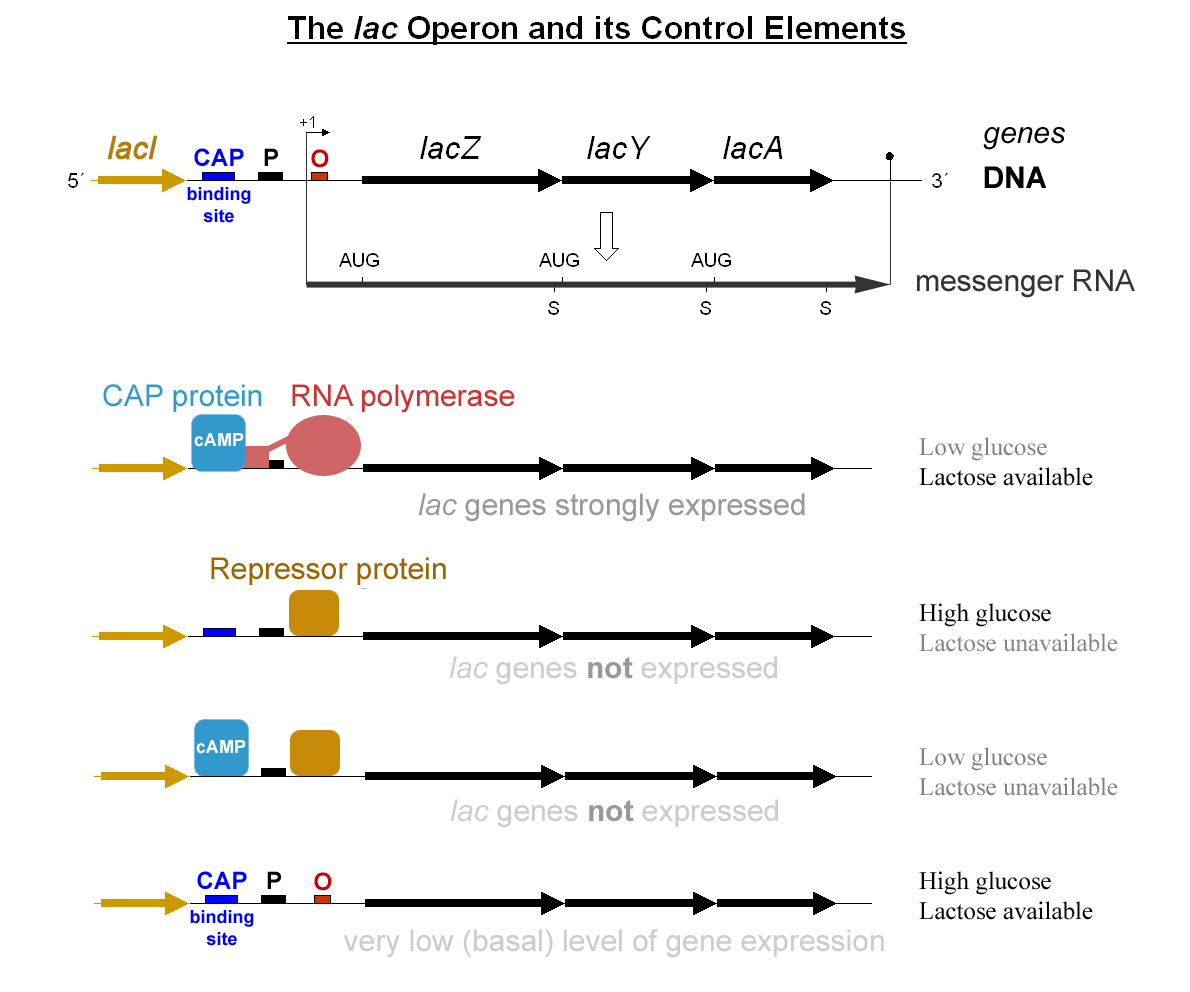
\includegraphics[width=\linewidth]{images/Lac_operon-2010-21-01.png}
    \caption[Exemple de l'opéron lactose]{Schéma du fonctionnement de l'opéron lactose. Sur la partie haute est représenté la structure génétique de l'opéron. Les 4 lignes suivantes représentent chacune une configuration de réponse à des conditions de présence, absence de glucose et de lactose. si le taux de glucose est faible, une protéine activatrice (CAP) va se fixer en amont du promoteur pour aider à la fixation de l'ARN polymérase, et si du lactose est disponible, les gènes seront alors fortement exprimés. Si le lactose n'est pas disponible, une protéine de répression va se fixer à l'opérateur et elle empêchera l'ARN polymérase de se fixer même si le taux de glucose est faible. 
    Auteur : G3pro. Sous licence Creative Commons 2.0. Disponible à l’adresse : \url{https://commons.wikimedia.org/wiki/File:Lac_operon-2010-21-01.png.}
    }
    \label{fig:lac_operon}
\end{figure}


%L'opéron, découvert par François Jacob et Jacques Monod en 1960\footnote{Découverte qui leur a valu le prix Nobel de médecine en 1965}\cite{jacob_operon_2005}, correspond à un ensemble de gènes (dits structuraux) qui vont être transcrits en une seule molécule d'ARNm. Cet ARNm va ensuite être traduit en plusieurs protéines, qui sont généralement impliquées dans le même processus. L'intérêt de cette structure réside dans une régulation coordonnée de la production de protéines, limitant le coût métabolique pour l'organisme. L'exemple le plus connu (et le premier) est celui de l'opéron lactose (\autoref{fig:lac_operon}). 3 gènes, \textit{lacA}, \textit{lacY} et \textit{lacZ}, sont traduits en 3 protéines\footnote{\textit{lacZ} code la $\beta$-galactosidase, \textit{lacY} code la $\beta$-galactoside perméase, \textit{lacA} code la $\beta$-thiogalactoside acétyltransférase.} fonctionnant ensemble pour catalyser le lactose. Sur la \autoref{fig:lac_operon}, on voit que 2 mécanismes de régulation collaborent pour réguler l'expression. Le premier au niveau du promoteur avec la protéine CAP, qui aide à la fixation de l'ARN polymérase, qui en l'absence de glucose ne se fixe pas au promoteur. Le second au niveau de l'opérateur qui en l'absence de lactose voit une protéine de répression se fixer sur lui et qui empêche la fixation de l'ARN polymérase. L'expression des gènes de l'opéron sont donc réguler pour répondre à 4 conditions environnementales différentes.

Pour terminer, l'expression des gènes peut aussi être régulé par le niveau de repliement et de condensation de l'ADN. L'ADN est condensé notamment grâce à des protéines appelées histone et à la méthylation de l’ADN. L'ADN replié ne pourra pas être accessible pour la transcription des gènes et donc ils seront inactifs. Les mécanismes liés à la méthylation de l'ADN sont l'affaire de l’épigénétique. Des études récentes ont mis en lumière le rôle de la méthylation dans la régulation de la virulence bactérienne et dans la capacité des procaryotes à coloniser leurs hôtes \cite{oliveira_bacterial_2021}, soulignant ainsi l'importance de ces mécanismes dans la survie et l’adaptation des bactéries.

\subsection{Îlots génomiques}
\label{sec:ilot}
Les îlots génomiques (GI, pour \textit{Genomic Island en anglais}) chez les procaryotes sont des régions spécifiques du génome qui jouent un rôle clé dans l'évolution, l'adaptation et l'acquisition de fonctions spécifiques. Les GIs sont retrouvés chez quasiment tous les organismes procaryotes. Ils sont généralement acquis par transfert horizontal (cf. \autoref{sec:evo_hz}) et transportent des gènes accessoires. Ils vont conférer à l'organisme de nouvelles fonctions qui impacteront de façon positive sa \textit{fitness}. Le premier îlot génomique détecté était lié à la capacité de la bactérie \textit{E. coli} de provoquer des maladies et a donc été nommé îlot de pathogénicité \cite{hacker_deletions_1990}.  Depuis, d'autres classes d'îlot ont été décrites : métabolique, résistance, symbiotique\dots (\autoref{fig:GI}).

Les îlots génomiques sont des régions assez larges, entre 5 et 200 kb (mais certaines sont beaucoup plus grandes) et présentent des caractéristiques spécifiques. (\textit{i}) Les GIs ont un taux de GC qui différe par rapport au reste du génome, résultant en un biais d'usage des codons\footnote{Un biais d'usage des codons, désigne la fréquence d’utilisation préférentielle de certains codons parmi les codons synonymes pour coder un même acide aminé.} (\autoref{fig:GI}). (\textit{ii}) dans les régions flanquantes des GIs, on retrouve des gènes de mobilité : transposases et intégrases, mais aussi d'IS qui peuvent se dégrader rapidement après l'intégration de l'îlot. (\textit{iii}) Dans les gènes flanquant, on retrouve des gènes codant l'ARNt dont l'origine serait à relier à la prévalence des gènes de phages et des ICEs qui utilisent les ARNt comme site d'intégration dans les génomes \cite{dobrindt_genomic_2004}. (\textit{iv}) Les protéines contenues dans les GIs ont souvent des fonctions inconnues. (\textit{v}) Dans la partie flanquante, on trouve des séquences répétées directes\footnote{Séquences identiques présentes en plusieurs copies dans la même molécule d'ADN et ayant la même orientation.}.

\begin{figure}[htbp]
    \centering
    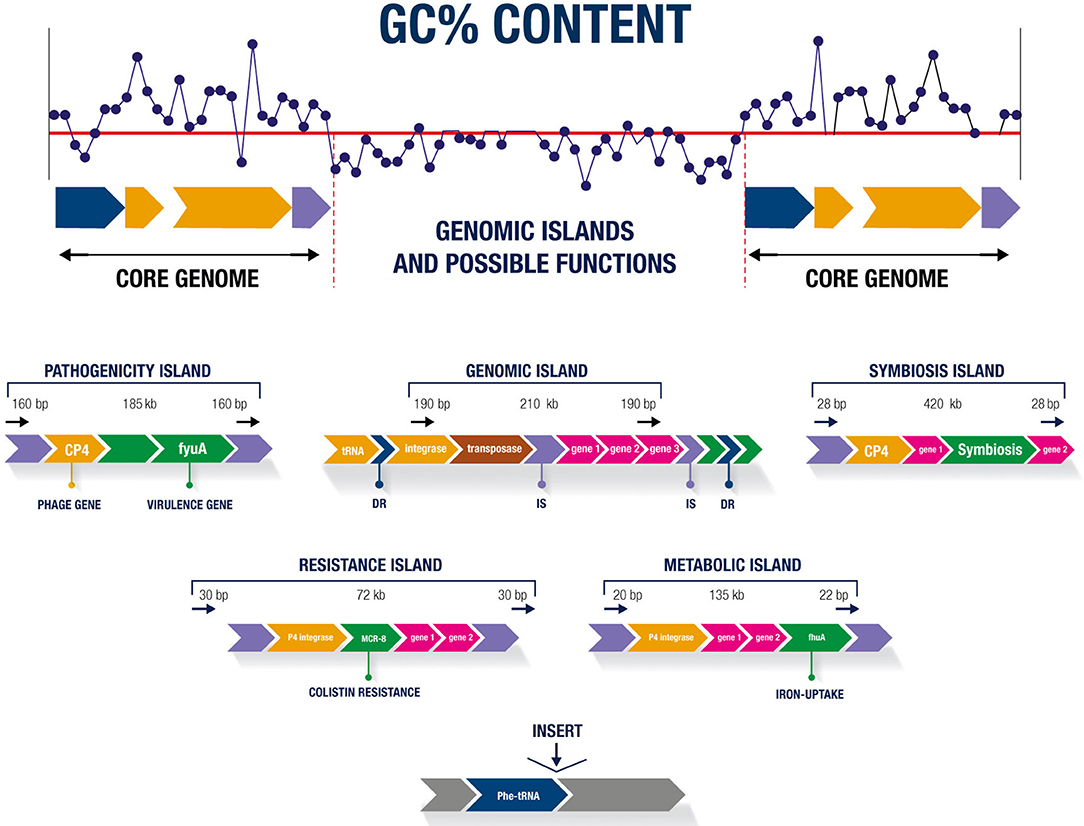
\includegraphics[width=0.8\linewidth]{images/ilot_genomique.jpg}
    \caption[Îlots génomiques et leur caractéristique]{Îlots génomiques et leur caractéristique \cite{da_silva_filho_comparative_2018}}
    \label{fig:GI}
\end{figure}

Ces GIs sont complexes à étudier, car ils peuvent être très différents entre les génomes, même proches. L'histoire évolutive est souvent difficile à reconstituer, tant des éléments ont été intégrés et éliminés au cours du temps (\autoref{fig:cycle_IG}). En plus de s'échanger avec d'autres organismes \cite{buchrieser_high-pathogenicity_1998}, les GIs pourraient se déplacer au sein du génome \cite{karaolis_bacteriophage_1999}. Ces caractéristiques rendent en théorie caduque certaines hypothèses comme le lien entre proximité spatiale et fonction. 

\begin{figure}[htbp]
    \centering
    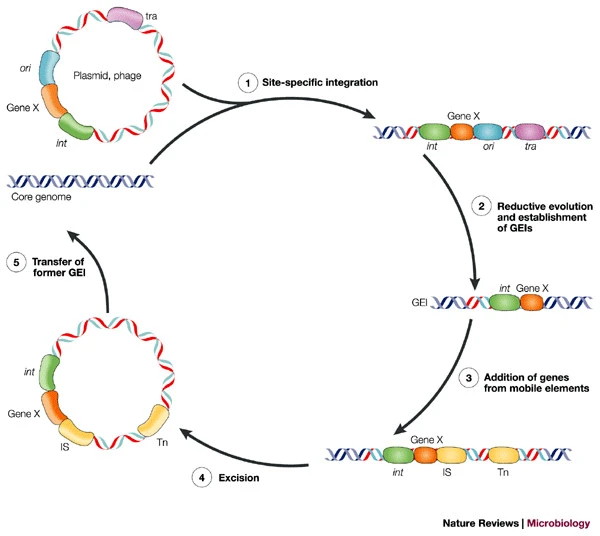
\includegraphics[width=0.8\linewidth]{images/cycle_GI.png}
    \caption[Cycle de vie d'un îlot génomique]{Cycle de vie d'un îlot génomique. Extrait de \cite{dobrindt_genomic_2004}}
    \label{fig:cycle_IG}
\end{figure}